
\begin{figure}[t]%
\centering
\parbox{2.5in}{

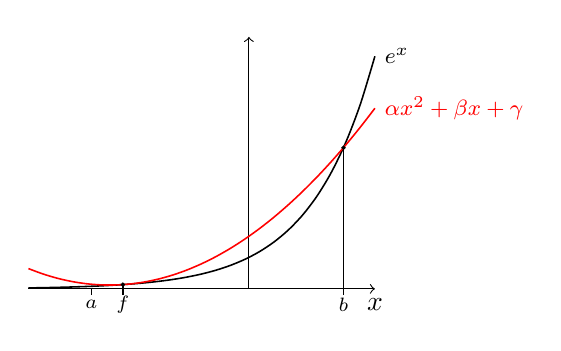
\begin{tikzpicture}[scale=0.8]
\draw[->] (-3.5,0) -- (2,0) node[anchor=north] {$x$};
\draw[->] (0,0) -- (0,4) node[anchor=east] {};
\draw[smooth, domain=-3.5:2.0, color=black, line width=0.20mm] 
    plot (\x,{e^(\x)/2}) node [right] {\footnotesize $e^x$};
\draw[smooth, domain=-3.5:2.0, color=red, line width=0.20mm] 
    plot (\x,{(0.316137167001903*\x*\x + 1.39988395124422*\x + 1.67055451771745)/2}) node [right] {\footnotesize $\alpha x^2+\beta x+\gamma$};
\draw (1.5,-0.1) -- (1.5,{e^(1.5)/2});
\draw (-2,-0.1) -- (-2,{e^(-2)/2});
\draw (-2.5,-0.1) -- (-2.5,0);
\draw[black,fill] (1.5,{e^(1.5)/2}) circle (0.25mm);
\draw[black,fill] (-2,{e^(-2)/2}) circle (0.25mm);
\draw	(-2.5,-0.25) node{{\scriptsize $a$}}
		(-2,-0.25) node{{\scriptsize $f$}}
		(1.5,-0.25) node{{\scriptsize $b$}};
\end{tikzpicture}

\caption[A parabola touching and intercepting an exponential curve]{A parabola parametarised by touching and intercepting points $f,b$ above an exponential curve for all $a\le x\le b$}%
\label{fig:graph1}}%
\qquad
\begin{minipage}{2.5in}%

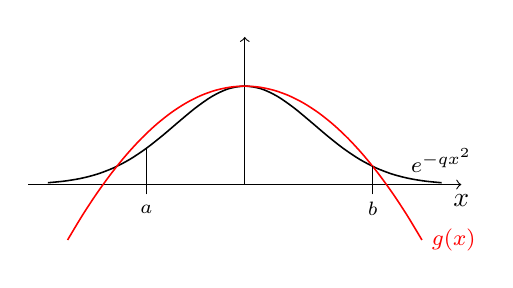
\begin{tikzpicture}[scale=1.25]
\draw[->] (-2.2,0) -- (2.2,0) node[anchor=north] {$x$};
\draw[->] (0,0) -- (0,1.5) node[anchor=east] {};
\draw[smooth, domain=-2.0:2.0, color=black, line width=0.20mm] 
    plot (\x,{e^(-(\x*\x))}) node [above] {\footnotesize $e^{-qx^2}$};
\draw[smooth, domain=-1.8:1.8, color=red, line width=0.20mm] 
    plot (\x,{-0.4825*\x*\x+1}) node [right] {\footnotesize $g(x)$};
\draw (1.3,-0.1) -- (1.3,{e^(-1.3*1.3)});
\draw (-1,-0.1) -- (-1,{e^(-1*1)});
\draw	(-1,-0.25) node{{\scriptsize $a$}}
		(1.3,-0.25) node{{\scriptsize $b$}};
\end{tikzpicture}

\caption[A parabola above a gaussian curve]{$g(x)=(e^{-qd^2}-1)d^{-2}x^2+1$ over function $f(x)=e^{-qx^2}$ for all $a\le x\le b$ where $d=\max(b,-a)$}%
\label{fig:graph111}%
\end{minipage}%
\end{figure}
